\begin{problem}{/images/problems/28_grid.png}{find the treasure}You are given an $11 \times 11$ table, a cell of which contains a treasure. Every time we can choose a  rectangle from the table and ask an oracle whether the treasure is in the rectangle. The oracle then responds with a ``Yes" or a ``No". What is the minimum number of questions we need to ask from the oracle in order to find the treasure?\\[0.2cm]

Link to the problem on Twitter:  \url{https://twitter.com/Riazi_Cafe/status/1693859687786074266}\end{problem}
\begin{solution}
The answer is 7.\\[0.2cm]

Because we divide the search space into two parts with each question, and we start with $11^2 = 121$ candidates the answer cannot be less than $\lceil \log 121\rceil=7$. Let us start by explaining a simple solution with 8 questions, and then we show how we can find the treasure with 7 questions.

If, inspired by binary search, we divide the main rectangle into 2 almost equal rectangles each time and ask one of them, we will find the treasure with at most 8 questions: First we ask if the treasure is in a  $11\times 6$ rectangle, then a $6\times 6$ rectangle, then a $3 \times 6$ rectangle, then a $3 \times 3$ rectangle, then a $3 \times 2$ rectangle, then a $2 \times 2$ rectangle, then a $2 \times 1$ rectangle, and finally a $1 \times 1$ rectangle. An example is shown in the figure below.

\begin{center}
	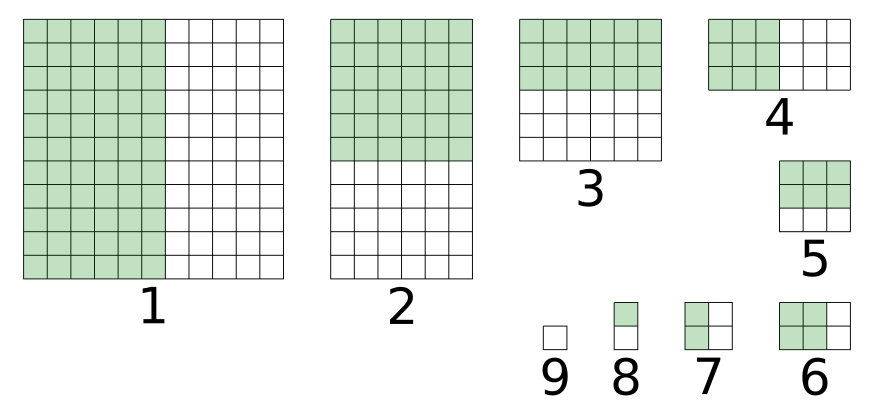
\includegraphics[width=14cm]{/images/problems/28_diagram0.png}
\end{center}

In order to improve our strategy, we make two observations:
\begin{itemize}
\item In order to keep the number of questions bounded by 7, after the first question, a maximum of 64 cells must remain in the search space; after the second question, a maximum of 32 cells. More formally, after the $i$'th question, the number of cells remaining in the search space should be at most $2^{7-i}$. In the above solution, after the first question, we may end up with 66 cells in the search space which does not lead to a solution with 7 questions.
\item The cells remaining in the search space do not have to be connected.
\end{itemize}

In our solution, we ask if the treasure is in the  red rectangle first, as shown below. Let us first consider the case where the answer is ``No" and explain the other case later. If the answer is ``No", our second question will be for the green rectangle in right figure. By these two questions, we limit the search space to a maximum of 61 cells in the first question and to a maximum of 31 cells in the second question. 

\begin{center}
	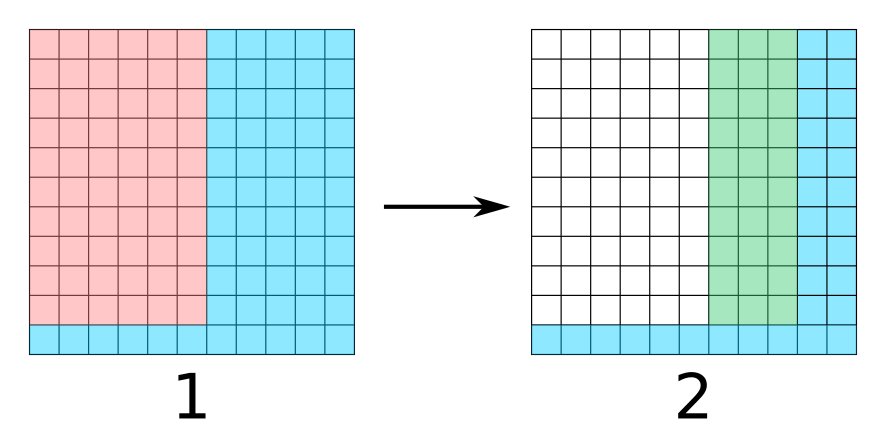
\includegraphics[width=9cm]{/images/problems/28_diagram1.png}
\end{center}


 We will postpone the ``Yes" case of the second question to later. If the answer to the second question is ``No", then 31 cells remain in the search space. In this case, by asking the black and white part of the figure below, we divide the search space into 2 parts of 15 cells and 16 cells.  After this question, we can divide the search space into two pars of equal size (with a difference of at most one) in each step and thus we can find the treasure with a maximum of 7 questions in total.

\begin{center}
	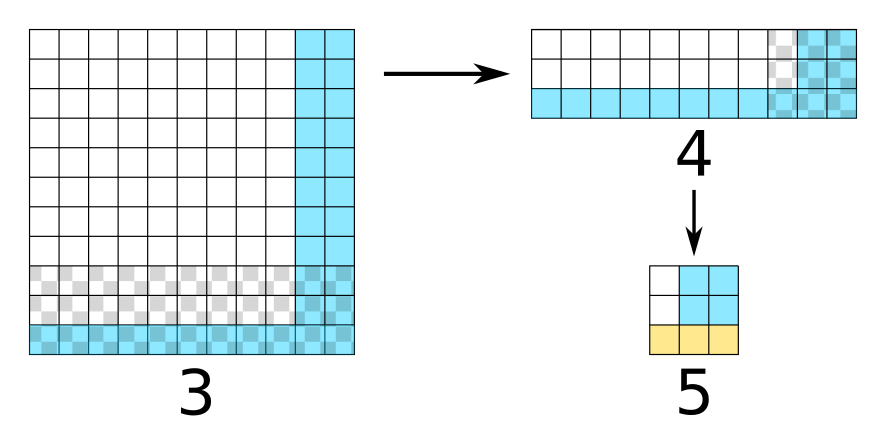
\includegraphics[width=9cm]{/images/problems/28_diagram2.png}
\end{center}

 
 What remains is to explain the solution when the treasure is in the red rectangle of the first figure or the green rectangle of the second figure. With two questions for the red rectangle and one question for the green rectangle the space of search can be narrowed down to a  $3 \times 5$ rectangle. After this, we only need four more questions to find the treasure as explained in the figures below. 
 
\begin{center}
	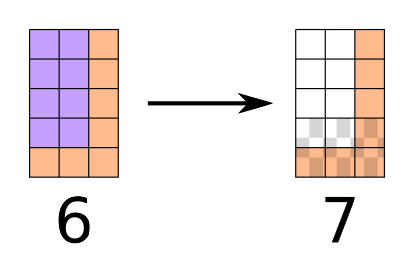
\includegraphics[width=9cm]{/images/problems/28_diagram3.png}
\end{center}

\end{solution}
